\documentclass[border={1cm 1cm 1cm 1cm}]{standalone}

\usepackage{tikz}

%Result of a Series of Wave Fronts Passing the Edge of a Wall
%Taylor, Rupert. (1970). Noise. New York: Penguin

%there's a deeper mathematical pattern here, but I can't see it yet.

\begin{document}
	
	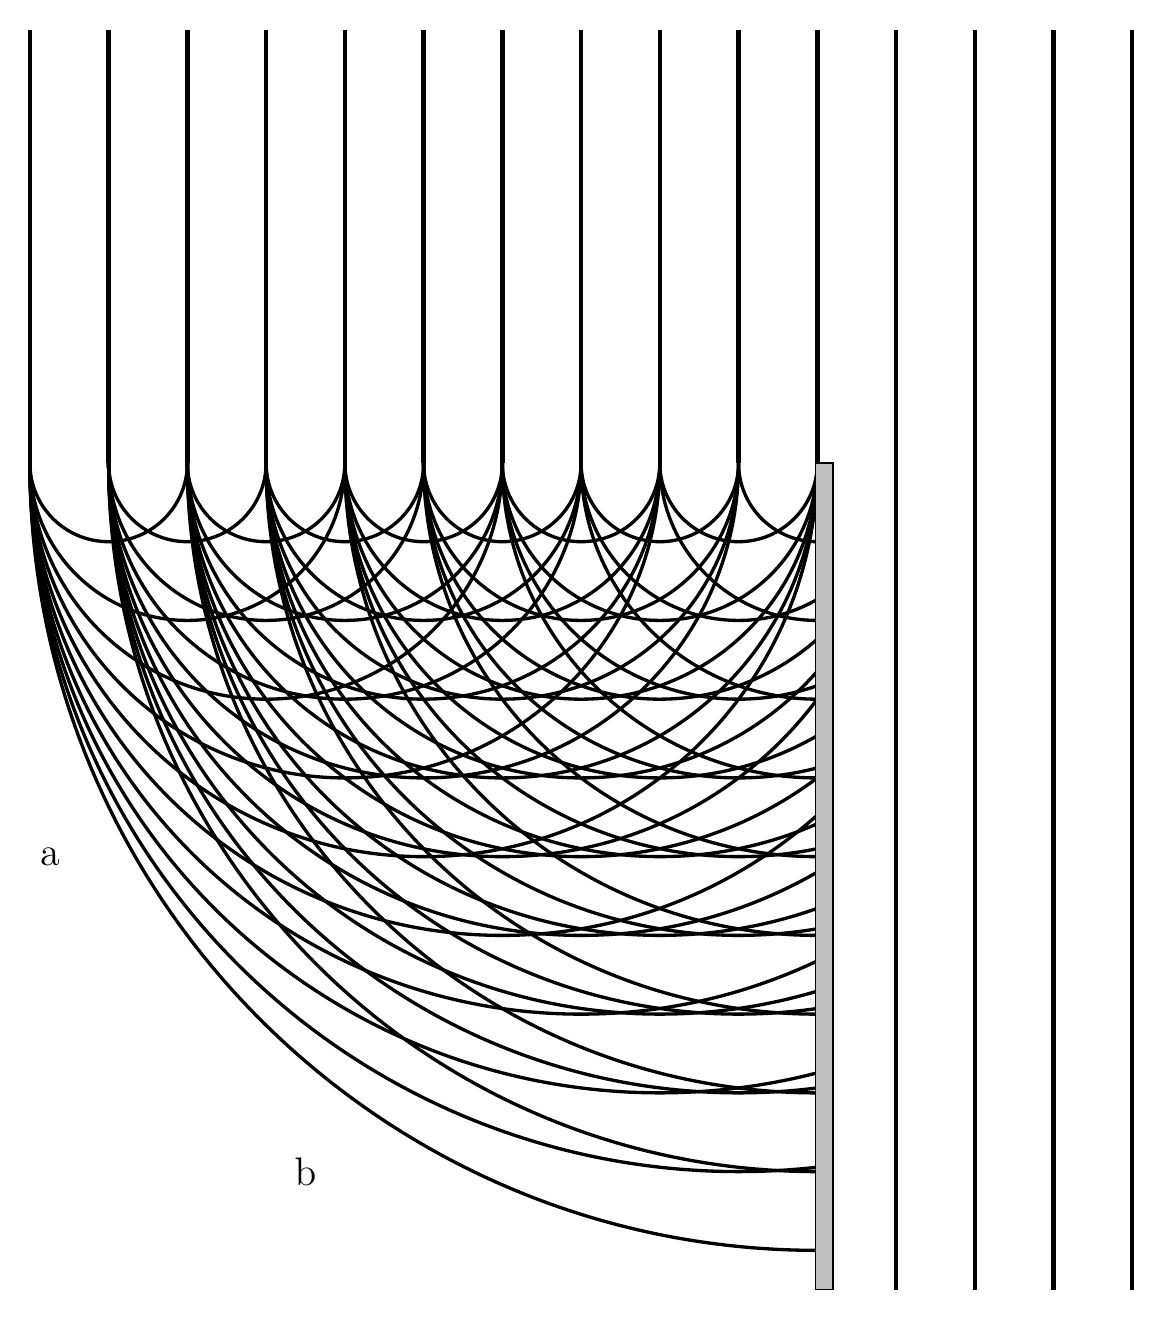
\begin{tikzpicture}
	%semicircles
	\foreach \x in {0,...,8}{
		\draw[very thick] (\x,0) arc (180:360:1cm);}
	\draw[very thick] (9,0) arc (180:270:1cm);					%straggler at the end
	
	\foreach \x in {0,...,6}{
		\draw[very thick] (\x,0) arc (180:360:2cm);}
	\draw[very thick] (7,0) arc (180:300:2cm);					%270+(3/4)^0*30
	\draw[very thick] (8,0) arc (180:270:2cm);
	
	\foreach \x in {0,...,4}{
		\draw[very thick] (\x,0) arc (180:360:3cm);}
	\draw[very thick] (5,0) arc (180:270+1.85*0.75^1*30:3cm);
	\draw[very thick] (6,0) arc (180:270+0.85*0.75^1*30:3cm);	%22.5 = (3/4)^1*30
	\draw[very thick] (7,0) arc (180:270:3cm);
	
	\foreach \x in {0,...,2}{
		\draw[very thick] (\x,0) arc (180:360:4cm);}
	\draw[very thick] (3,0) arc (180:270+2.9*0.75^2*30:4cm);
	\draw[very thick] (4,0) arc (180:270+1.8*0.75^2*30:4cm);
	\draw[very thick] (5,0) arc (180:270+0.85*0.75^2*30:4cm);	%16.875 = (3/4)^2*30
	\draw[very thick] (6,0) arc (180:270:4cm);
	
	\draw[very thick] (0,0) arc (180:360:5cm);
	\draw[very thick] (1,0) arc (180:270+4.2*0.75^3*30:5cm);	%breaks the pattern - why?
	\draw[very thick] (2,0) arc (180:270+2.9*0.75^3*30:5cm);
	\draw[very thick] (3,0) arc (180:270+1.85*0.75^3*30:5cm);
	\draw[very thick] (4,0) arc (180:270+0.9*0.75^3*30:5cm);	%12.62625 = (3/4)^3*30
	\draw[very thick] (5,0) arc (180:270:5cm);
	
	\draw[very thick] (0,0) arc (180:270+4.4*0.75^4*30:6cm);	%new pattern emerges
	\draw[very thick] (1,0) arc (180:270+3.15*0.75^4*30:6cm);
	\draw[very thick] (2,0) arc (180:270+2.05*0.75^4*30:6cm);
	\draw[very thick] (3,0) arc (180:270+1.025*0.75^4*30:6cm);	%1 + 1.025^1/(4-\x)  <--nope
	\draw[very thick] (4,0) arc (180:270:6cm);
	
	\draw[very thick] (0,0) arc (180:270+3.55*0.75^5*30:7cm);	%3.5 is too short
	\draw[very thick] (1,0) arc (180:270+2.3*0.75^5*30:7cm);
	\draw[very thick] (2,0) arc (180:270+1.15*0.75^5*30:7cm);
	\draw[very thick] (3,0) arc (180:270:7cm);					%7.11914 = (3/4)^5*30
	
	\draw[very thick] (0,0) arc (180:270+2.7*0.75^6*30:8cm);
	\draw[very thick] (1,0) arc (180:270+1.35*0.75^6*30:8cm);
	\draw[very thick] (2,0) arc (180:270:8cm);
	
	\draw[very thick] (0,0) arc (180:270+1.6*0.75^7*30:9cm);
	\draw[very thick] (1,0) arc (180:270:9cm);
	
	\draw[very thick] (0,0) arc (180:270:10cm);
	
	%vertical lines
	\foreach \x in {0,...,10}{
	\draw[ultra thick] (\x,5.5)--(\x,0);}
		\filldraw[fill=lightgray] (9.98,0) rectangle (10.2,-10.5);
	\foreach \x in {11,...,14}{
		\draw[ultra thick] (\x,5.5)--(\x,-10.5);}
	
	\node at (0.25,-5)  {\Large a};
	\node at (3.50,-9)  {\Large b};
	\end{tikzpicture}
	
\end{document}